%Comment this line out to use real graphics instead of demo boxes.  Do not use \usepackage[demo]{graphicx} because that causes
%conflicts with other packages with dependencies.
%\PassOptionsToPackage{demo}{graphicx}

\RequirePackage{fix-cm}

\documentclass[numbook, envcountsect, envcountsame, envcountreset, runningheads, twocolumn]{svjour3}
%\usepackage{fullpage}%Don't use with IEEEtran
\usepackage[titletoc, title]{appendix}
\usepackage{amsmath}
\usepackage[version=3]{mhchem}
\usepackage{url}
\usepackage{cite}
\usepackage{graphicx}
\usepackage{threeparttable}
%\usepackage{caption}%Don't use with IEEEtran
%\usepackage{subcaption}%Don't use with IEEEtran
\usepackage{color}
%\usepackage{lscape}%Resist using
%\usepackage{natbib}%Don't use with IEEEtran
\usepackage{pdfpages}
\usepackage{listings}
\usepackage{multirow}
\usepackage[super]{nth}
\usepackage{siunitx}
\usepackage{setspace}
\singlespacing
\usepackage{microtype}
\usepackage{soul}
\newcommand{\angstrom}{\textup{ \AA}}
\newcommand{\degree}{$^{\circ}$}

\usepackage{fp}
\usepackage{calc}
\usepackage{color}
\usepackage{soul}





%SINGLES
\newcommand\costonepcb{33}

%COMM. BOARD
\newcommand\costcparts{130.72}
\newcommand\costcpartc{168.51}
\newcommand\costcasyms{0}
\newcommand\costcasymc{0}
\newcommand\costsclcpcb{491.04}
\newcommand\costsclcasyms{40.31}
\newcommand\costsclcasymc{99.2}
\newcommand\costsclcparts{0}
\newcommand\costsclcpartc{0}

%SENS. BOARD
\newcommand\costsparts{51.13}
\newcommand\costsasym{0}
\newcommand\costsclspcb{186.99}
\newcommand\costsclsasym{13.49}
\newcommand\costsclsparts{0}


%SENSORS
\newcommand\costoneMQ{0}
\newcommand\costoneK{85.00}
\newcommand\costoneGC{0}
\newcommand\costonelex{0}
\newcommand\costonepump{0}
\newcommand\costsclMQ{0}
\newcommand\costsclK{0}

%CELL. BOARD
\newcommand\costcellpart{204.06}
\newcommand\costsclcellpcb{0}
\newcommand\costsclcellpart{204.06}

%TYCON
\newcommand\costonetycsm{165.56}
\newcommand\costonetyclg{1099.95}
\newcommand\costscltycsm{165.56}
\newcommand\costscltyclg{1099.95}


%MAGIC COMMANDS - DO NOT TOUCH
% Counters for totaling up hours and dollars
\newcounter{cost}
\setcounter{cost}{0}
% Formats inputed number with 2 digits after the decimal place
\newcommand*{\formatNumber}[1]{\FPround{\cost}{#1}{2}\cost} %
% Returns the total of counter
\newcommand*{\total}[1]{\FPdiv{\t}{\arabic{#1}}{1000}\formatNumber{\t}}
% Adds up multiple counters
\newcommand*{\additup}[1]{%
	\addtocounter{cost}{1000 * \real{#1}}}%	

%SUMS
\newcommand\costsumone{
	\setcounter{cost}{0}
	\additup{\costonepcb}
	\additup{\costcparts}
	\additup{\costcasyms}
	\additup{\costonepcb}
	\additup{\costsparts}
	\additup{\costsasym}
	\additup{\costoneMQ}
	\additup{\costoneK}
	\additup{\costonetycsm}
	\total{cost}
	}
\newcommand\costsumtwo{
	\setcounter{cost}{0}
	\additup{\costonepcb}
	\additup{\costcparts}
	\additup{\costcasyms}
	\additup{\costonepcb}
	\additup{\costsparts}
	\additup{\costsasym}
	\additup{\costoneMQ}
	\additup{\costoneK}
	\additup{\costoneGC}
	\additup{\costonelex}
	\additup{\costonepump}
	\additup{\costonepcb}
	\additup{\costcellpart}
	\additup{\costonetyclg}
	\total{cost}
	}
\newcommand\costsumthr{
	\setcounter{cost}{0}
	\additup{\costsclcpcb}
	\additup{\costsclcparts}
	\additup{\costsclcasyms}
	\additup{\costsclspcb}
	\additup{\costsclsparts}
	\additup{\costsclsasym}
	\additup{\costsclMQ}
	\additup{\costsclK}
	\additup{\costscltycsm}
	\total{cost}
	}
\newcommand\costsumfou{
	\setcounter{cost}{0}
	\additup{\costsclcpcb}
	\additup{\costsclcpartc}
	\additup{\costsclcasymc}
	\additup{\costsclspcb}
	\additup{\costsclsparts}
	\additup{\costsclsasym}
	\additup{\costsclMQ}
	\additup{\costsclK}
	\additup{\costoneGC}
	\additup{\costonelex}
	\additup{\costonepump}
	\additup{\costsclcellpcb}
	\additup{\costcellpart}
	\additup{\costonetyclg}
	\total{cost}
	}


\graphicspath{ {images/} } %this removes clutter from the root folder

\smartqed % flush right qed marks, e.g. at end of proof

\begin{document}
	\title{Description of a Wireless, Remote-Sensing Array for Detection of Carbon Dioxide and Methane Gas Leaks Near the Atmospheric Baseline}
	\titlerunning{Description of Remote-Sensing Array for Detection of CO$_{2}$ and CH$_{4}$ Leaks}
	
	\author{Wesley T. Honeycutt \and
		Nicholas F. Materer \and
		M. Tyler Ley
	}
	
	\institute{W. Honeycutt \at
		Department of Chemistry, Oklahoma State University, 107 Physical Sciences, Stillwater, OK 74078, USA \\
		\email{wes.honeycutt@okstate.edu} \\
		\emph{Present address:} of W. Honeycutt \at
		Oklahoma Biological Survey, University of Oklahoma, 111 Chesapeake St., Norman, OK 73019, USA
		\and
		N. Materer \at
		Department of Chemistry, Oklahoma State University , 107 Physical Sciences, Stillwater, OK 74078, USA \\
		\email{materer@okstate.edu}
		\and
		T. Ley \at
		College of Engineering, Architecture and Technology, Oklahoma State University, 201 ATRC, Stillwater, OK 74078, USA \\
	}

	\date{Received: date / Accepted: date}
	% The correct dates will be entered by the editor

	\maketitle
	
	\begin{abstract} 
		This abstract is abstract.
		%Springer Only
		\keywords{Chemical sensors \and
			Gas industry \and
			Pollution measurement \and
			Spectroscopy \and
			Carbon \and
			Chemistry \and
			Gas detectors \and
			Sensor systems and applications}
		% \PACS{PACS code1 \and PACS code2 \and more}
		% \subclass{MSC code1 \and MSC code2 \and more}
	\end{abstract}
	
	\section{Introduction}
	
		The effect of carbon dioxide in the atmosphere on terrestrial temperature has been known to science since the late \nth{19} century as quantified by Arrhenius~\cite{arrhenius_xxxi._1896}.  As carbon dioxide output from anthropogenic sources increases~\cite{boden_global_2011}, it becomes increasingly important to find solutions to prevent excessive buildup.  One such proposed solution is injection of excess carbon dioxide underground.  There, the injected gas can be stored in naturally occurring subterranean voids or those left by mining and hydrocarbon extraction processes.  Alternately, the carbon dioxide can be used as an extraction fluid to pull valuable hydrocarbons such as methane still remaining in these wells in a process termed Enhanced Oil Recovery (EOR).  Sites of particular interest are bituminous sands, unreachable coal beds, deep saline aquifers, and salt caverns~\cite{bachu_sequestration_2000, white_separation_2003}.  
		
		In sequestration efforts, carbon dioxide is collected and pressurized from significant waste streams such as those produced by coal-fired power plants, and injected into underground voids~\cite{white_separation_2003}.  It is theorized that the majority of the injected gas will be converted from fluid carbon dioxide to carbonate salts with time after the injection.  By this process, the waste streams from large industrial producers of carbon dioxide is converted from an emitted greenhouse gas pollutant to a more manageable solid form.  As it is accepted that the injected carbon dioxide will remain underground for many years, it is considered to be a viable solution to excess emissions.  In a secondary process, as the carbon dioxide seeps from the storage depth, it undergoes biogenic reduction to methane, an even more potent greenhouse gas~\cite{romanak_process-based_2012}. Most of this gas is expected to remain in the storage site as well, but reliable sensing method for detecting problems due to changes in flux of both these gases is essential to the safe deployment of this method in the interest of environmental health and safety.  Studies comparing the collection and injection methods of the gas into different storage locations at small scale suggest that carbon sequestration by the injection of flue gas into underground voids is a net benefit in terms of greenhouse gas mediation efforts~\cite{khoo_life_2006}.  
		
		%\begin{figure}[h!]
		%	\centering
		%	\includegraphics[width=\columnwidth,height=0.8\columnwidth,keepaspectratio]{process.png}
		%	\caption[A summary of carbon dioxide injection wells]{This diagram shows a simplified explanation of the carbon dioxide injection process.  The cartoon depicts carbon dioxide being collect from a large industrial source, e.g. a power plant, and pumped into a deep saline aquifer well.  The gas is injected as a supercritical fluid near the top of a void surrounded by a sturdy rock formation.  The pressure from the expanding fluid pressurizes the well.  Remaining oil in the well sitting in a layer above the aquifer is easily pumped out by existing infrastructure.}
		%	\label{fig:process}
		%\end{figure}
		
		The pressurized carbon dioxide gas can be used to liberate hydrocarbons from the ground by treating the gas as an extraction solvent rather than a permanent injectable.  This is the premise of the use of carbon dioxide injection as a method of enhanced oil recovery (EOR).  Pressurized carbon dioxide is pumped into new or existing wells and the fluid fills in spaces in the surrounding earth, replacing an existing material which is easily dissolved into the carbon dioxide~\cite{chadwick_latest_2009} and potentially liberating valuable gases trapped in these underground areas such as methane~\cite{white_sequestration_2005}.  Most EOR projects occur at existing oil and gas developments or at ``depleted'' sites~\cite{cook_what_2014}.  A report from the National Energy Technology Laboratory of the United States Department of Energy claims that the sequestration of 20 billion metric tons of carbon dioxide has been employed as part of EOR programs since their discovery~\cite{kuuskraa_improving_2011, kuuskraa_co2_2013}.  As of 2014, 53\% of all commercial-scale EOR projects in the United States utilize gas injection techniques, and the number of projects using this method is expected to increase as there is more push for carbon dioxide sequestration in conjunction with rising energy prices~\cite{manrique_eor_2006}. Unlike environmental remediation sequestration efforts, the majority of the carbon dioxide gas for EOR projects is pumped from geologic sources, rather than captured waste streams.  Only a third of the gas used in small-scale EOR research wells was procured from flue gas~\cite{cook_what_2014}.
		
		There are some concerns regarding the potential outcomes of such storage regimes~\cite{kharaka_potential_2009}.  A large leak of the sequestered carbon dioxide which has not undergone conversion to carbonate salts has the potential for catastrophic and expensive consequences.  A plume of carbon dioxide has the potential of suffocating all animal life in an area, as evidenced by the events at Lake Nyos~\cite{kling_1986_1987} and Lake Monoun~\cite{sigurdsson_origin_1987} in Cameroon which caused massive loss of human life.  It is essential that this outcome be avoided, therefore it is equally essential to monitor the gas flux from the storage sites over time.  
		
		Small leaks over time, while less catastrophic in nature, would undermine the assumption that carbon sequestration as a fail-proof storage mechanism for excess carbon dioxide waste gas as the presumed net gain in environmental health would be lost over longer periods.  There have been no studies of carbon dioxide leakage from carbon sequestration sites over long time scales.  This is due, in part, to the recent development of the technique.  However, there are currently inadequate monitoring technologies for this kind of study.  Often, atmospheric ramifications of sequestration and EOR is ignored entirely.  Only half of small-scale EOR testing projects conducted atmospheric monitoring, instead most rely on subsurface monitoring and geochemical modeling techniques~\cite{cook_what_2014}.
		
		If the fluidized carbon dioxide in the rocky subsurface environment can be thought of as a mobile phase in a large solid substrate, it is reasonable to suspect that voids in the solid material would physically separate as layers.  It is proposed by some researchers that the injected carbon dioxide will migrate towards the surface, eventually seeping out in small quantities, in a process known as microseepage~\cite{klusman_baseline_2005, klusman_rate_2003, carrroll_geochemical_2009}.  This is the vertical migration of an underground ``plume'' which moves toward the surface.  This plumed gas eventually will leak from the subterranean storage site from small fissures in the ground.  
		
		%\begin{figure}[!t]
		%	\centering
		%	\includegraphics[width=\columnwidth,height=0.8\columnwidth,keepaspectratio]{plumegroup.png}
		%	\caption[The steps in subterranean plume migration]{This cartoon depicts a simplified illustration of the plume which forms during carbon dioxide injection.  In the leftmost image, a quantity of carbon dioxide is pumped in from the surface (represented somewhat inaccurately by the oil derrick).  As more carbon dioxide is left in the well, the supercritical fluid expands through crevices in the rock and sediment layers predominantly toward the surface.  Eventually, this stored gas will reach the surface and begin to gradually seep out through a process known as microseepage.}
		%	\label{fig:plumegroup}
		%\end{figure}
		
		The migration of carbon dioxide is recognized as an important factor for determining the economic feasibility of an injection well as well as a prospective legislative issue~\cite{vandeweijer_monitoring_2011}.  It is difficult and costly to monitor these gas plumes experimentally.  Instead, researchers rely heavily on computer modeling, which has been shown to be effective for predicting the lateral diffusion of the plume underground~\cite{oldenburg_process_2001,zhang_gas_2016}.  The scope of many theoretical studies of carbon dioxide injection primarily focuses on lateral plume migration through individual layers, assuming that there is minimal vertical migration~\cite{singh_numerical_2012}.  While this is predominantly the case, moderately porous materials with interconnected channels induce gas mobility to a similar degree as inter-particulate spaces in laboratory testing~\cite{honari_enhanced_2015}.  Certain models for the prediction of plume migration after injection are simplified by assumptions which may not accurately model the physical world, including the assumption that the surface layer is impermeable to the fluidized gas~\cite{patel_high-fidelity_2016}.   Fluidized carbon dioxide does not increase porosity of solid material, however the focus on lateral plume migration in theoretical models does not adequately address the potential for microseepage from subterranean storage environments.
		
		\subsection{Current Monitoring Strategies}
		
			Monitoring of gas flux transitioning from subsurface storage areas to the atmosphere can take place using a variety of techniques at various locations around a wellhead and plume site.  Atmospheric monitoring methods include optical sensors such as non-dispersive infrared (NDIR), light detection and ranging (LIDAR), sorbent sampling of tracer molecules, and eddy covariance (EC) flux monitoring; near-surface monitoring methods include soil sampling, flux accumulation,  hyperspectral imaging, and many more~\cite{netl_best_2012}.  While this list is limited in scope, it touches upon some of the most commonly deployed strategies.  There is currently no option which allows for sensitive detection of analyte gases at a short time-scale with remote monitoring for long measuring periods.  The current implementation of these strategies ranges from being ineffective to outright hazardous.
			
			The relative inaccessibility of many injection well sites poses a problem.  Field site operators take either core samples or headspace samples from multiple sites in the area which are analyzed at other locations. This is difficult and inefficient.  There is a recent push to introduce more remote monitoring technologies to reduce these shortcomings.  Spectroscopy remains an ever attractive options for remote sensing of local gas concentrations.  Hyperspectral imaging, LIDAR, and other similar technologies working in combination have been shown to be powerful in detecting leak anomalies~\cite{bateson_application_2008, male_using_2009}, but require a trained operator to function.  The recent availability of unmanned aerial systems has been of particular interest for remote monitoring~\cite{salami_uav_2014}.  These systems only allow for temporary scanning, as planes must be refueled, batteries recharged, and sensors redeployed for each of these scans.  Continual monitoring of a site requires active maintenance.  Satellites in geosynchronous orbit allow for constant hovering above large areas.  A recent study by NASA of a methane leak has shown that the modern LIDAR equipment was even able to measure an above-ground gas plume from a large leak~\cite{thompson_space-based_2016}.  The gas leak depicted in the article by Thompson et al. was exceptionally large.  Most leak events and microseepage occurrences are minor deviations from the local baseline.  Current space based spectrometers cannot detect near-baseline deviations of small leakage sites.  Additionally, the deploying a satellite is still prohibitively expensive.  This means that continual monitoring of every potential leakage site is bottlenecked by the available satellites.  Custom built terrestrial remote monitoring stations in development for the In Sallah injection well have been shown to have strong detection capabilities in simulated leaks~\cite{barr_laser-based_2011,humphries_testing_2008}.  These proposed sensors are only capable of single site monitoring as of this publication.  As potential leakage from subterranean storage site may occur over a large area and from surrounding abandoned wells~\cite{nordbotten_model_2009,nordbotten_semianalytical_2005}, single site detection is not practical for monitoring of the large area potentially affected by an injected carbon dioxide plume.  Eddy Covariance is praised for the large area that can be monitored, however the devices are maintenance intensive, requiring adequate infrastructure in the sequestration area and computational power due to data complexity~\cite{klusman_comparison_2011}.  Current remote monitoring techniques may serve to reduce the man-hours required compared to traditional soil sampling regimes, yet they fall short of the desired goals of true remote detection of small local environmental changes.
			
			Possibly the most selective method for detecting flux of injected chemicals to the atmosphere is the use of tracer chemicals.  Addition of a trace quantity of an inert chemical is made during the injection process.  Sites can be monitored by selective testing for these chemicals.  The low signal-to-noise ratio of optical detection for tracer chemicals in flux gas is an attractive option, but has the potential for environmental damage by way the persistent pollutant nature of the perfluorocarbons used as tracers~\cite{wells_atmospheric_2013, wells_use_2007}.  For crude oil well-to-well analysis, it has long been established that the addition of an anthropogenic radioisotope can be detected from pumped material based on characteristic radiation from the sample.  Only certain chemicals meet the needs of carbon dioxide injection wells~\cite{craig_field_1985}.  Notable among this subset is the use of halogenated organic compounds, sulfur hexafluoride, and hydrogen sulfide.  Many of these chemicals have been identified as environmentally hazardous compounds.  Many of the halogenated organic compounds recommended for use, often freon variants, are persistent chemicals with high greenhouse gas potentials.  Sulfur hexafluoride, while attractive due to its inert qualities, is extremely persistent with high radiative forcing such that it is considered to be more than 26,000 times more greenhouse warming potential over the 100 years than carbon dioxide~\cite{myhre_2013:_2013}.  Some tracers, such as hydrogen sulfide, have been shown to enter aquifers, causing them to be non-potable sources for future use~\cite{apps_review_2006}.  These tracer chemicals may not even be effective in supercritical fluids.  It is proposed that higher solubility of carbon dioxide in water than tracer chemicals may lead to inaccurate concentration measurements in offshore injection environments and wells known to contain significant water deposits~\cite{vandeweijer_monitoring_2011}.  An optimal solution to the monitoring of injection wells would quantify the migrating gas without requiring an environmentally persistent tracer.  
			
			There are no monitoring devices which can collect data from multiple sites simultaneously over short time-scales over a continuous period.  This is evidenced by the lack of available data on the diel cycle of gas concentrations.  Isolated studies have been conducted which have established the day-night cycling of gases such as carbon dioxide and methane, yet these often only measure a few points of data per 24-hour cycle.  Determining the diel cycle for these gases is valuable to climate scientists, biologists, and agricultural engineers, and data of the diel cycle of concentration over various terrestrial and aquatic local environments is available in the literature for carbon dioxide~\cite{raymond_carbon_1997,goulden_diel_2004,raich_comparison_1990,osozawa_diel_1995,ni_sestructures_2000,maberly_diel_1996} and methane~\cite{ding_diel_2004,kaki_diel_2001,zhang_diel_2011,wang_effect_1997,wang_factors_1999,van_der_nat_diel_1998}.  While only a sampling of the available literature is mentioned in the previous citations, a critical analysis of all of these sources shows that current technologies are not utilized to detect concentration often, for a long time, and over a large area.  These studies usually involve a single sampling instrument operated continuously for a short period, samples taken with large gaps between points, or distributed detection of multiple sites not performed concurrently.  
			
			%Recent developments of devices under the ``internet of things'' notion suggest that construction of devices for this purpose should be simple.  Yet no one has done it.  The specialized knowledge required to construct these devices, the programming experience required to operate them, and the time required to perfect such devices to a field-deployable state appears to have deterred many scientists from attempting to create units of this class.  The construction and characterization of instruments designed for distributed detection in the scientific literature would provide a framework for other scientists-reducing the barrier to these technologies for applications described in this monograph as well as further applications.
			
			A technological niche exists for a relatively inexpensive device which can monitor a large number of sites easily with little human interaction.  A solution to this problem exists in the application of available technology to develop a distributed sensing unit that wirelessly transmits information to a gathering center.  This idea in itself is not completely without precedent.  Wireless sensor arrays have been used before in agricultural applications to monitor conditions~\cite{garcia-sanchez_wireless_2011} and aerial cloud analysis~\cite{allred_sensorflock:_2007}.  In these cases they have demonstrated the capacity to perform required monitoring functions over a large area with low cost and human interaction.  An adaptation of this technology to fit with the needs of gas monitoring at wellheads provides our solution.
			
			In this paper, the design and construction of the individual nodes of a networked array of sensors is described.  First, a simplified schematic of the network is offered and explained.  Next, the circuits employed by the sensors are described, including information about relevant breakout boards.  This paper explores the individual circuit design for power supply, processing and memory, xbee wireless communication, cellular communication, environmental sensors, small gas concentration sensors, larger pumped gas concentration sensors, and ground protection.  All relevant schematics are reported by the Honeycutt dissertation~\hl{Cite Wes Dissertation}.  The difference between the passive and active gas sampling regimes is discussed.  Finally, this paper relates the development of the prototype boards and movement into production of 110 units for deployment in the field.
		
		
	%%\FloatBarrier
	\section{Device Design}
		
		To best facilitate the collection and analysis of the data from remote sites, a tiered device hierarchy was created.  Most of the nodes were computationally simple, acting as end points of the network by collecting the data.  These sensor nodes require the gas sensors, light power supply hardware, and radio for simple wireless communication to other nodes.  The middle tier of the network collects data from the sensor nodes and communicates it to the next level.  These communication nodes are computationally simple much like the sensor nodes, but they spend more time and energy processing than the smaller sensor nodes.  Thus, the communication nodes require similar gas sensors and radio, but with a more robust power supply.  The coordinated data is transmitted to the upper level via cellular phone protocols, necessitating a cell modem.  With the extra power made available to the communication nodes, better quality sensors could be added to them, allowing verification of incoming data.  They employ a set of actively pumped sensors in addition to the passive sensors included in the smaller nodes.  The highest tier of the network would be a computational workstation housed at the base of operations.  This computer, connected to the municipal power supply, is stationary and can afford to have any number of configurations.  It acts as a receiver of the field data.  Data are sent to a web server being run by this workstation.  An organized list of requirements for the device hierarchy can be see in table~\ref{tab:hierarchy}.
		
		\begin{table}[!t]
			\centering
			\begin{tabular}{r | l}
				Tier and Name & Device Requirements\\
				\hline
				\begin{tabular}{r}
					Tier 0 \\
					Web Server
				\end{tabular} &
				\begin{tabular}{l}
					Large Storage Space
				\end{tabular} \\
				\hline
				\begin{tabular}{r}
					Tier 1 \\
					Communication Node
				\end{tabular} &
				\begin{tabular}{l}
					Simple gas sensors \\
					Advanced gas sensors \\
					Moderate power supply \\
					Wireless communication \\
					Cellular modem
				\end{tabular} \\
				\hline
				\begin{tabular}{r}
					Tier 2 \\
					Sensor Node
				\end{tabular} &
				\begin{tabular}{l}
					Simple gas sensors \\
					Low power supply \\
					Wireless communication
				\end{tabular} \\
			\end{tabular}
			\caption[Device hierarchy]{Hierarchy and respective requirements of devices in the network array designed for this project}
			\label{tab:hierarchy}
		\end{table}
		
		The nodes can be generalized as a set of functional units, such as depicted in Figure~\ref{fig:outline}.  The functional units are grouped as ``power'', ``Arduino based processing'', and ``glue electronics.''  Although the power supply capacity of each node on the tier differs, the power supervisor and supplies required for each unit are essentially the same.  The ``Arduino based processing'' parts are shared between tiers as well.  By producing similar board infrastructure on tiers 1 and 2, parts unique to a certain tier such as the cellular modem are added on as additional breakout parts to the central board.  The ``glue electronics'' may be expected to change for the more powerful sensors included with the communication nodes, but sensor redundancy in these nodes can work with the more powerful sensors used in addition to the simple ones.  These redundancies provide the advantage of comparing responses between the sensor types, providing calibration during the post-process. 
		
		\begin{figure}[!t]
			\centering
			\includegraphics[width=\columnwidth,height=\columnwidth,keepaspectratio]{outline.pdf}
			\caption[Equipment outline]{A generalized representation of the equipment to be included in each node.}
			\label{fig:outline}
		\end{figure}
		
		\subsection{Gas Sensors}
			
			Several commercially available carbon dioxide and methane sensors were selected and evaluated for applicability to the sensor array. A full description of sensors studied for this application, including those which have been employed in this build are discussed by Honeycutt et al.\hl{we need our first paper included here}  Certain sensor units were chosen for specific promised abilities.  Notably, the K-30 model from CO$_2$Meter was chosen and cheap, lightweight sensors which promised satisfactory detection of carbon dioxide.  The Gascard sensors sold by GHG Analytical were an order of magnitude more costly than the other sensors, but the advertised capability made them attractive enough to make up for the expense if only used on select units.  The MQ-4 methane sensor was chosen as the inexpensive methane detector; though it lacks the high sensitivity to concentration changes which the other sensors possess, it will serve to detect large shifts in the methane present.  Due to the unique interface requirements of each sensor unit, development kits were purchased when possible for prototyping.  
		
		
		\subsection{Power Management}
		
			The nature of the sensor array designed to cover a relatively large area of land imposes limitations upon the power supply of the system.  Since the area to be covered may include elevation changes, anthropogenic developments, and other uncontrollable factors, it would not be convenient to constrain the array by wired connection as the array will be adapted to individual site conditions.  Therefore, each unit must be designed with internal and self-sustaining power supplies.  Two different types of commercially available solar power generation and storage units with weatherproof enclosures were selected from Tycon Power Systems.  The majority of the sensors would be housed in the Remote Pro \SI{2.5}{\watt} Continuous Remote Power System die cast enclosure (Figure~\ref{fig:enclosure}~A) and a few sensor units with features requiring more power were housed in the Remote Pro \SI{15}{\watt} Continuous Remote Power System steel enclosure (Figure~\ref{fig:enclosure}~B).  The \SI{2.5}{\watt} enclosure includes a \SI{12}{\volt} battery rated for \SI{9}{\ampere\hour} of use, a charging and distribution circuit, and a \SI{10}{\watt} solar panel.  The \SI{15}{\watt} enclosure includes a \SI{12}{\volt} battery pair rated for a combined \SI{98}{\ampere\hour}, a charging and distribution circuit, and a \SI{60}{\watt} solar panel \cite{tycon_power_systems_remotepro_2014}.  
			
			\begin{figure}[!t]
				\centering
				\includegraphics[width=\columnwidth,height=0.8\columnwidth,keepaspectratio]{enclosures.png}
				\caption[Tycon Power Systems enclosures]{The (A) Remote Pro 2.5 W Continuous Remote Power System and (B) Remote Pro \SI{15}{\watt} Continuous Remote Power System\textendash{}image from Tycon Power Systems' website shows typical units.}
				\label{fig:enclosure}
			\end{figure}
			
			%The individual sensors were tested with a Fluke 179 True RMS Multimeter to ascertain the current and voltage across the power leads to verify the values provided in the specifications for each part.  The calculated power from each of these measurements is summarized in the first part of Table~\ref{tab:componentpower}.
			
			During prototyping of the devices using readily available Arduino development boards, the power consumption of units were found to quickly outstrip the combined charging and storage of power by the solar cells and batteries.  The Arduino prototype was found to use \SI{2.7}{\watt} of power, which was higher the continuous use rating of \SI{2.5}{\watt} for the small enclosure power system.  By subtracting the sensor power from the total consumption of the Arduino prototype, it was determined that the Arduino circuitry was too power intensive for this application.  Thus it became clear that a dedicated power supply circuit would need to be designed for the deployed units.  
			
			Furthermore, monitoring the capacity of the manufacturer supplied batteries showed a tendency for them to decay over time.  The enclosure units include an automated circuit for trickle charge of the batteries by the solar cells and an automatic shutoff of power supplied to electronics included by the user if the battery voltage drops below \SI{10.7}{\volt}.  Based on repeated discharge tests to this cutoff voltage depicted in Fig.~\ref{fig:batterydecay}, the shut down threshold is too low for the batteries and may potentially require repairs of deployed field units.  To correct this, a voltage monitoring circuit was added to the control boards.  The microcontroller program allows for the unit to automatically detect user specified threshold voltages, and preempts the manufacturer supplied shutoff circuit.  
			
			\begin{figure}[!t]
				\centering
				\includegraphics[width=\columnwidth,height=0.8\columnwidth,keepaspectratio]{decay.pdf}
				\caption[Battery Decay with Repeated Discharge]{Repeated discharge of the batteries during multiple tests showed that the battery capacity was lost over time when used in conjunction with the manufacturer supplied trickle charge module.}
				\label{fig:batterydecay}
			\end{figure}
		
	%\FloatBarrier
	\section{Circuit Description}
		
		Figure~\ref{fig:board} shows the control board as designed with all components included.  This board is included in all of the high level communication nodes in the network.  Sensor nodes use the same printed circuit board, but do not have electrical components included for unit parts not incorporated into the sensor nodes, such as the Gascard sensor and cellular modem.  
		
		\begin{figure}[!t]
			\centering
			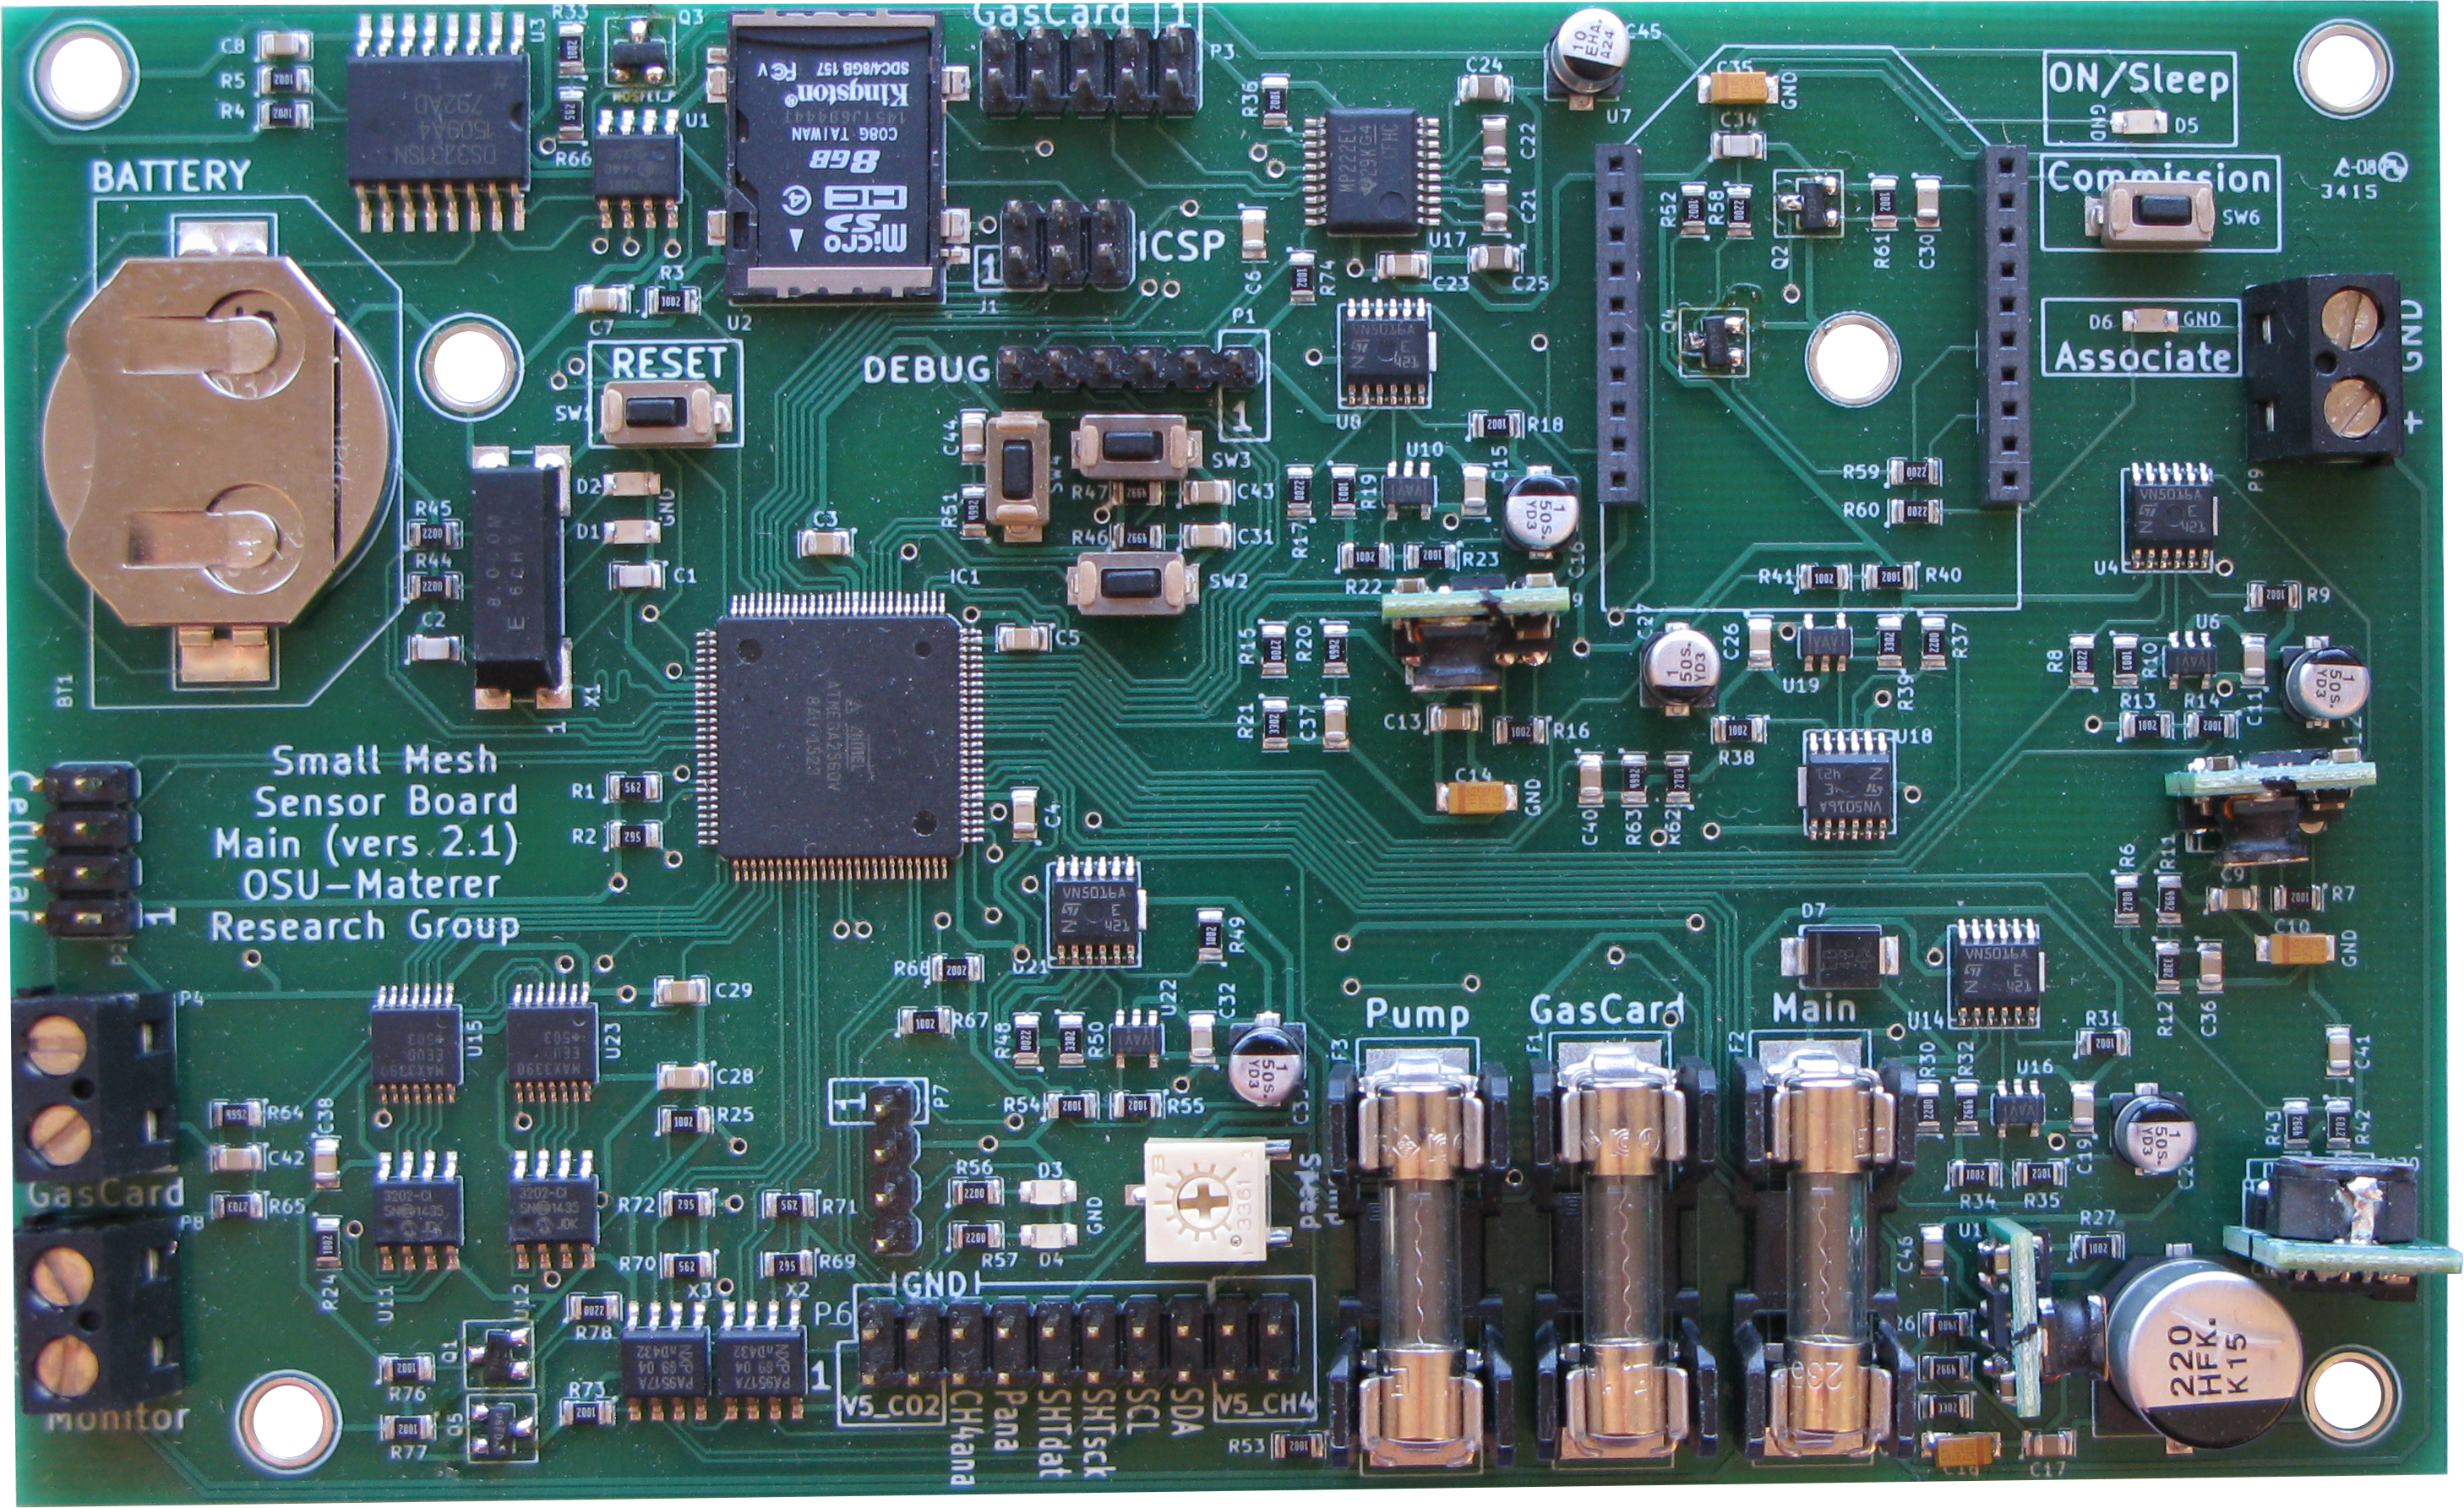
\includegraphics[width=\columnwidth,height=0.8\columnwidth,keepaspectratio]{commboard.png}
			\caption[Control board]{The fully built communication node command board designed for this study.}
			\label{fig:board}
		\end{figure}
		
		The sensor command module was designed in such a way as to minimize wasted power.  A selection of parts considered for use in the board were measured for current and voltage to determine their power use.  The control board designed for this project uses \SI{1.7}{\watt} during full use.  To prepare for times when the solar panel cannot provide continuous charging, a problem which can last for long periods in the deployment area, 32\% of the year is at least half-cloudy and 8\% of the year is heavily overcast~\cite{kswo_weather_2015}. A lower power use mode was programmed.  The control board can select a medium mode which reduces the frequency of sampling by some of the more energy expensive sensors.  This is automatically triggered by the control program if the battery charge is determined to be at 70\% charge.  A hibernation mode was also programmed.  This mode disables the sensors, communication circuitry, and microprocessor, leaving only power supply and real-time clock connected to the circuit.  Below a certain battery voltage threshold, the unit can hibernate to prevent complete power drain, and it will restart again once the battery registers above the threshold voltage.  Using only \SI{0.1}{\milli\watt} during hibernation, this mode prevents the units from requiring manned intervention during inclement conditions.
		
		%Power Supply
		\subsection{Power Supply}
			The unit is powered from the case supply circuit through 22 AWG wire connected via terminal block.  This \SI{12}{\volt} line goes through a \SI{1}{\ampere} cartridge fuse and powers several circuits.  The \SI{12}{\volt} line sends power to a \SI{3.3}{\volt} DC/DC converter circuit, two separate \SI{5}{\volt} DC/DC converter circuits, and the power supply for the Gascard (for the larger communication nodes only).  The \SI{3.3}{\volt} power is supplied by the \SI{12}{\volt} line through a Murata Power Solutions OKI-78SR-33/1.5-W36-C fixed output \SI{1.5}{\ampere} DC/DC converter.  The \SI{5}{\volt} power is supplied by a more complex circuit, depicted in Fig.~\ref{fig:zoom03}.
			
			\begin{figure}[!t]
				\centering
				\includegraphics[width=\columnwidth,height=0.8\columnwidth,keepaspectratio]{zoom03.pdf}
				\caption[Circuit - 5 V Dc/DC converter circuit]{The \SI{5}{\volt} DC/DC converter circuits run the \SI{12}{\volt} line from the battery (Vbatt) through a STMicroelectronics VN5016AJ-E single channel high side driver which delivers current of a clamped voltage to components further downstream.  The high side driver is switched by a current sense input.  When this current sense is low, the current delivered by the chip is proportional to the load current based on a known ratio.  The current of the voltage clamp is passed through a Texas Instruments TLV2471IDBVR \SI{600}{\micro\ampere} \SI{2.8}{\mega\hertz} rail-to-rail input/output high drive operational amplifier which is operating as a closed loop non-inverting amplifier.  Status is reported to the microcontroller (ADCO2).  The high side driver delivers the power to the input of a Murata Power Solutions OKR-T/1.5-W12-C adjustable output \SI{1.5}{\ampere} DC/DC converter (POSLOGIC12).  This device efficiently converts power between \SI{0.591}{\volt} and \SI{6}{\volt} based on trim, and it may be turned off when a separate pin is pulled low.  The power delivered to the unit by the high side driver is used to pull the on/off pin high with a \SI{10}{\kilo\ohm} resistor.   The calculated resistance required for the trim pin to achieve \SI{5.00}{\volt} is \SI{268}{\ohm}.  A \SI{270}{\ohm} resistor was determined to produce voltage within bounds of the requirements for the components powered by this converter without requiring an expensive non-standard resistor value.  The \SI{5}{\volt} line produced by the converter is monitored by the ATmega 2560 microcontroller on an A/D pin protected by resistors (AD2).}
				\label{fig:zoom03}
			\end{figure}
		
		%ATmega 2560
		\subsection{Processor and Memory}
			The board commands are coordinated by an Atmel ATmega 2560 lower power 8-bit microcontroller with 64 kB flash operating on a RISC architecture (referred to as ATmega 2560 in this manuscript).  The ATmega 2560 is connected to a MA-506 \SI{8}{\mega\hertz}$\pm$30 ppm crystal oscillator with equivalent length traces.  Several push-button switches with associated LEDs are connected directly to the controller to act as human interface for simple commands such as reset, on/off, and dump log.  Interface with the RISC architecture can occur through either a TTL/RS-232 header or an in-circuit serial programming header for programming firmware or debugging.  These headers connect directly to the ATmega 2560 and do not pass through any RS-232 type translators.  
			
			Logging is managed by the controller using timestamps from a DS3231 real-time clock.  The real time clock uses a CR-2016 coin cell battery to maintain correct count of the date.  Data can be logged using two memory storage methods.  The first is 24LC1026 1024 kB serial EEPROM.  The second is a micro Secure Digital stable storage inserted into an Alps SCHD3A0100 micro SD card holder which is activated by a Vishay Si2377EDS p-type MOSFET connected to the ATmega 2560 chip.
			
		%Xbee
		%%\FloatBarrier
		\subsection{XBee Wireless Communication}
			Communication of the nodes with the rest of the mesh occur by way of an XBee wireless device.  For this application, the XBee-Pro 900HP model was chosen.  This \SI{900}{\mega\hertz} radio module is capable of data transfer rates of up to 200 kbps with \hl{impressive range}, depending on the antenna gain.  The XBee communicates directly with the ATmega 2650 chip via TX/RX serial communication.  Traces also directly connect with the board to send signals telling the radio to reset and sleep.  The circuit has some human interface components.  One LED provides ``on'' status, a pushbutton switch is set to the ``commission'' function of the XBee firmware, and another LED is tied to the ``associate'' function.  The commission button allows the user to wake a device, send node identifying codes, broadcast a request to join a network, and restores default values depending on the number of times the button is pressed.  The associated LED provides information about the status of the network and diagnostics which can be interpreted by the rate and number of blinks by the diode.  The device is powered by the \SI{3.3}{\volt} power line, and the sleeping of the modem is controlled by this same power line.  When power begins flowing through the \SI{3.3}{\volt} line from an OFF state, an On Semiconductor 2N7002E n-type MOSFET sends a signal to the XBee to activate it.  A signal can be sent from the XBee to reset to ATmega 2560 as well. The signal is delayed slightly by a capacitor before another n-type MOSFET sends a signal to the control board with the reset signal.
			
		%Cellboard
		\subsection{Cellular Communication}
			\label{sec:cellsection}
			Communication by the control nodes to the data collection site takes place over cellular phone lines.  A breakout board is connected to the control board by a ribbon patch cable.  The breakout board houses a NimbeLink Skywire EVDO cellular modem.  The cellular modem requires a stable \SI{4}{\volt} power supply, so a dedicated power circuit was designed.  Much in the same way the other power supply circuits were constructed, this line draws the \SI{12}{\volt} from the battery to a VN5016AJ-E high side driver with switched current sensing using a TLV2471IDBVR op-amp to monitor the current at this point, similar to the \SI{5}{\volt} power supply depicted in Fig.~\ref{fig:zoom03}.  The power is converted using a similar Murata OKR-T/1.5-W12-C DC/DC converter with a \SI{348}{\ohm} resistor dialing in the output voltage required for the modem.  Monitoring of the power supply and switch is processed by the ATmega 2560.  The cellular modem is powered by the \SI{4}{\volt} power line, but a reference voltage to the input/output lines is also required.  Since the controller uses \SI{3.3}{\volt}, this reference voltage needs to reflect that.  The modem communicates with the ATmega 2560 by TX/RX serial port.  Two input output lines from the control board connect to n-type MOSFETs.  These act as switches to send signals to the modem for on/off and sleep operations.  
			
		%Sensorboard and sensor related circuitry
		\subsection{Sensor Breakout Board}
			While the communication nodes have more powerful sensors than the end nodes, all types share a set of the inexpensive sensors housed on a breakout board (Fig.~\ref{fig:sensorboardpic}).  Data are transfered to and from the control board by a 20 pin header connected by ribbon cable with power supply and ground cables.  Power lines in this cable use two wires each to prevent wire failure.  Several ground wires are used on the cable, positioned such that they alternate with the signal wires on the ribbon to prevent interference between lines.  The K series carbon dioxide sensor is powered by a \SI{5}{\volt} power line and communicates with the controller via I$^2$C SDA/SDL port.  \hl{omitted text commented out in \LaTeX code, see notes for discussion}
			
			
			% REMOVED TEXT
			%
			%The I$^2$C is translated through an NXP PCA9517A level translating repeater to shift the low voltage signals, which is limited by an internal resistor, up to the \SI{5}{\volt} signal which matches the input voltage.  This part was originally intended to shift the voltage from the \SI{3.3}{\volt} I$^2$C output from the K-series sensor.  As the design progressed, the microcontroller requirement was discovered to be \SI{3.3}{\volt} input.  Due to the timeline of the project, the sensor boards were already printed with the level translator to convert the signal to \SI{5}{\volt}.  A separate level converter on the main board converts the signal back down to \SI{3.3}{\volt}.  This part of the circuit is vestigial.  If one part of the device is changed in future versions, this grandfathered circuit may prove useful once again.    
			%
			% DISCUSSION
			%
			% This text was removed since it does not add to the narrative of the paper.  However, it is factually correct.  I suggest omitting it since we are not showing the circuit in this paper or the appendices, so we don't need to bring it up.  your input is welcome - WTH 07/10/17
			
			
			\begin{figure}[!t]
				\centering
				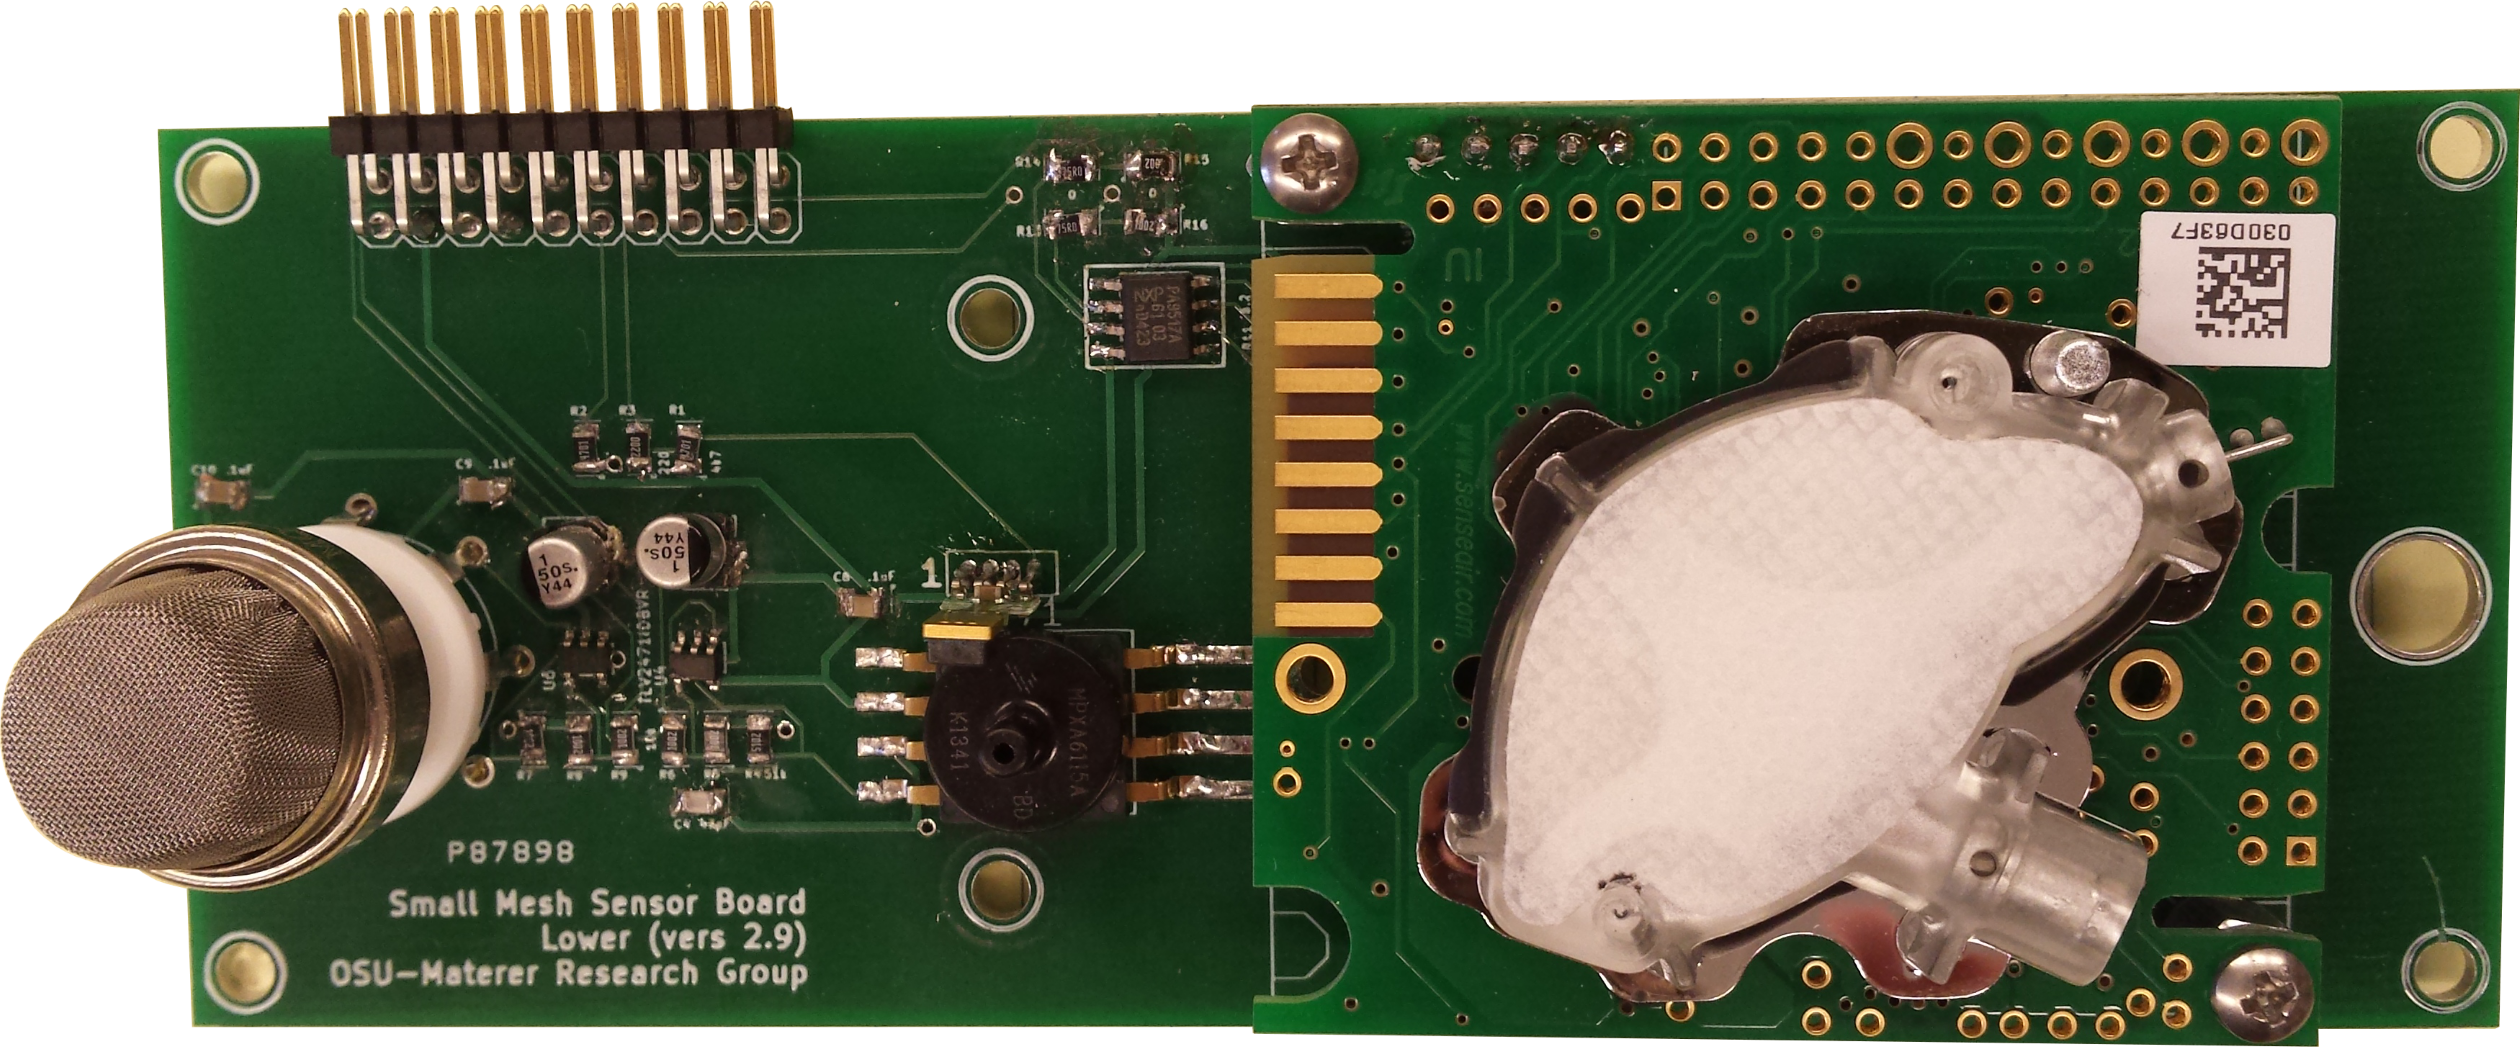
\includegraphics[width=\columnwidth,height=0.8\columnwidth,keepaspectratio]{sensorboardpic.png}
				\caption[Sensor breakout board]{A picture of the sensor breakout board with encapsulating materials removed.}
				\label{fig:sensorboardpic}
			\end{figure}
			
			The MQ-4 methane sensor is mounted on the board by connecting it to a special MQ socket for the MQ series of gas sensors.  The pin which connects to the heating coil of the MQ-4 sensor is powered by a dedicated \SI{5}{\volt} power line.  The two other input pins on the MQ-4 sensor connect to the primary \SI{5}{\volt} power line.  These pins are connected after the sensor and pulled down by a \SI{10}{\kilo\ohm} resistor before connecting to an op-amp.  The op-amp is configured as a closed loop non-inverting amplifier to boost the analog signal output by the sensor.  On the mainboard, the analog signal from the methane sensor is routed to a Maxim MCP3202 12 bit A/D converter with SPI.  The MCP3202 splits the analog signal into a digital component with comparison to a reference clock signal produced by the microcontroller, and it can be shutdown with a signal from the controller to reduce power consumption.  Digital output from the A/D converter and digital input to it must pass through a Maxim MAX3390E low-voltage level translator.  This converts the \SI{5}{\volt} signal used by the sensors to the \SI{3.3}{\volt} signal used by the ATmega 2560.  The tri-state outputs of this level translator minimizes the current used by the chip in the translation, an important feature for power conscious design.  
			
			Two gas property sensors are connected to the board.  The first is a Sensiriron SHT75 humidity and temperature sensor.  This device contains the amplifier, A/D converter, and memory necessary for operation.  The device is connected to the main board with only a few resistors such as a \SI{4.7}{\kilo\ohm} pull up on the data line, a \SI{4.7}{\kilo\ohm} pull down on the clock input line, and a \SI{220}{\kilo\ohm} resistor on the data line to resist inrush current on the long wire to the microcontroller.  On the main board side, the clock input is switched and inverted by a MOSFET (Figure~\ref{fig:zoom17}) and the data line is adjusted to the \SI{3.3}{\volt} input of the microcontroller by a PCA9517A level translator.  The second is a Freescale MPXA6115AC6T1 absolute, integrated pressure sensor.  Since this sensor package includes the circuitry to integrate the signal, all that is left to do on the circuit board is to boost the signal with an op-amp closed loop non-inverting amplifier circuit.  
			
		%Gascard
		\subsection{Gascard Implementation}
			The larger communication nodes have an additional sensor, the Edinburgh Gascard, for calibration purposes which has increased power requirements compared to the low power sensors.  This sensor has several dedicated circuits for its operation.  The Gascard operates under \SI{12}{\volt} conditions, the same as is supplied by the battery, negating the need for a DC/DC converter.  The power supplied by the battery passes through a VN5016AJ-E high side driver which is used to clamp the voltage and monitor the current output, amplified by a TLV2471IDBVR op-amp.  The output of the high side driver is fused to protect the circuitry and connects to a terminal block header.  A separate lead from the fuse, which is protected by resistors, is used to monitor the voltage output.  
			
			Unlike the membrane sensors used in the sensor nodes, the Gascard requires flow to operate.  All sensors used in the communication nodes will therefore be operating through flow enclosures.  This flow is produced by a Thomas 1410D/2.2/E/BLDC diaphragm pump.  The pump is powered by the \SI{12}{\volt} line and uses the same fused high side driver and op-amp circuit as the Gascard (Figure~\ref{fig:zoom21}).  The pump is connected by a four pin header.  Two of the pins are connected by a Bourns 3361P-1-103GLF potentiometer.  This Cermet trimpot can be adjusted from \SI{10}{\ohm} to \SI{10}{\kilo\ohm}, and it is used to adjust the speed of the pump.  
			
			Data communication to and from the Gascard occurs by means of a 10 pin header which connects the board to the sensor by ribbon cable.  Communication with the microcontroller is translated through a Texas Instruments MAXRS3222 multichannel RS-232 line driver/ receiver integrated circuit which translates the serial output of the Gascard to an asynchronous communication protocol (Figure~\ref{fig:zoom22}).  The IC is configured for operation at \SI{3.3}{\volt}, using \SI{0.47}{\micro\farad} capacitors on the charge pump capacitors.  These capacitors are larger than the minimum required by the circuit, but the increased capacitance will reduce ripple current on the transmitter outputs, decrease power consumption, and prevent equivalent series resistance issues.  The receive and transmit lines of the serial serial connection to the microcontroller are connected to the receiver output and driver input on the chip, respectively, and the serial receive and transmit coming from the Gascard connect to the driver output and receive input on the chip.  A digital input/output line from the microcontroller connects to a shutdown pin on the IC which is pulled down.
			
		%Capacitors
		\subsection{Ground Protection}
			Many components of the board are protected by capacitors to ground.  This is to prevent AC power fluctuations on DC subcircuit lines.  The capacitor allows the AC signal component to take the preferred path to ground by high frequency inductance while forcing DC signal to still go to the intended location.  Various capacitors are used for this application in the circuit including \SI{10}{\micro\farad} \SI{25}{\volt} rated electrolytic capacitor with 20\% tolerance, \SI{1}{\micro\farad} \SI{50}{\volt} rated electrolytic capacitor with 20\% tolerance, \SI{1}{\micro\farad} \SI{25}{\volt} rated tantalum capacitor with 10\% tolerance, \SI{0.1}{\micro\farad} \SI{25}{\volt} rated multilayer ceramic capacitor (MLCC) with 10\%tolerance, \SI{0.47}{\micro\farad} \SI{50}{\volt} rated MLCC with 10\% tolerance, and \SI{47}{\pico\farad} \SI{100}{\volt} rated MLCC with 5\% tolerance.  The values are selected to filter out noise expected from that signal.  Many of the values were selected based on manufacturer recommendations for the associated components.  Larger capacitors were chosen to eliminate sustained voltage drops, while the smaller capacitors were chosen to eliminate fast transient noise.  A tantalum capacitor was used in applications that required a larger capacitor with low reactance.  Multiple decoupling filters are used in series on lines where a wide range of signal noise may be encountered.
			
	%\FloatBarrier
	\section{Air Sampling}
	
		Samples of the ambient air at the field site are collected by both the small sensor nodes and the large communication nodes.  To minimize the power expenditure, the small nodes are set to passively sample the environmental conditions.  The large nodes have greater power storage capabilities, so these units sample the conditions by active sampling.  
		
		%Passive Sampling
		\subsection{Passive Sampling}
			The passive sampling method requires the sensor components to be directly exposed to the environment.  Placing an exposed circuit board into the relatively harsh conditions of the field site invites potential issues from moisture causing corrosion, animal life interfering with the fragile components, and damage from collisions.  To mediate this problem, a plastic housing to isolate the sensor components from the circuit boards and power supply electronics was constructed.  Sensors were placed in such a manner that they would have contact with the environment through holes pre-drilled on the enclosure.  These holes are oriented towards the ground to prevent collection of rainwater and moisture.  
			
			The plastic housing was designed in OpenSCAD, a free 3D computer aided design (CAD) program which renders a 3D object from a script file~\cite{kintel_openscad_2011}.  The interface objects were printed by i.materialise on an EOSINT P 700 by selective laser sintering of polyamide granules.  The manufacturer specifications for this printer also claim a \SI{100}{\micro\meter} layer resolution, depending on the source material used. 
			
			An isolating enclosure for the temperature and pressure sensors is mounted flush against the PCB and the void is filled with an epoxy potting compound (Fig.~\ref{fig:3d5}).  Enough of the potting compound is injected into this hole to cover the leads of the pressure and temperature sensors within without overfilling and preventing these sensors to operate.  This effectively seals the sampling areas which are exposed to the environment, off from interior of the enclosure.  No potting compound is necessary for the carbon dioxide sensor, as the extra bottom added to the cube compresses the outer edge of the membrane on that sensor and forms a satisfactory seal.  When the combined sensor circuit board and plastic part are attached to the enclosure, a small amount of silicone is applied to the flat surface of the plastic part, and the piece easily slips into the correct position on the enclosure (see Figure~\ref{fig:3d6}).  Due to problems with small invertebrates making homes in the sensor holes during the prototyping phase, a \SI{1}{\milli\meter} mesh screen is glued over the holes before the units were deployed.
			
			\begin{figure}[!t]
				\centering
				{\includegraphics[width=.8\columnwidth,height=0.8\columnwidth,keepaspectratio]{3d5.png}}
				\caption[3D printed part]{3D printed part ready to be inserted into the enclosure.\label{fig:3d5}}
			\end{figure}
			
			\begin{figure}[!t]
				\centering
				{\includegraphics[width=.8\columnwidth,height=0.8\columnwidth,keepaspectratio]{3d6.png}}
				\caption[3D printed part joins]{The custom part joins the sensor board and enclosure perfectly.\label{fig:3d6}}
			\end{figure}
		
		%Active Sampling
		\subsection{Active Sampling}
			\label{sec:activesampling}
			The larger power reserves in the communication nodes allow active sampling of the environmental conditions.  A Thomas 1410D/2.2/E/BLDC diaphragm pump pulls air from outside of the controller through a hole on the underside of the enclosure, through a \SI{0.45}{\micro\meter} particle filter, to the pump diaphragm.  Air is pushed out from the pump to a small plastic housing with the sensors that are used on the node sensors, then through the Gascard, and finally vented outside the enclosure.  Since it was essential to use the same sensor board in the communication node as is used in the sensor nodes to enable direct comparison of results, special consideration was needed to adapt the passive sampling sensors for the flow mode in units with active sampling.  To do this, a plastic housing was designed to hold the sensor board (see Figure~\ref{fig:lexbox}).  
			
			\begin{figure}[!t]
				\centering
				\includegraphics[width=.8\columnwidth,height=0.8\columnwidth,keepaspectratio]{lexbox.jpg}
				\caption[Lexan box housing]{Lexan box housing sensor board for use in communication nodes.  The box has been sealed from external flow by dichloromethane solvent at the joins.}
				\label{fig:lexbox}
		\end{figure}
		
	%\FloatBarrier
	\section{Prototyping}
	
		Early iterations of the sensor board were based on the Arduino interface circuitry developed during sensor selection.  This eliminated the need to develop a communications board before the sensor board as assembly plans were developed.  The Arduino setup allowed for the sensor board to be tested for correct operation of each sensor during the development phase and provide quality control for each of the 150 completed sensor board units.  To parallel the tests performed in laboratory setting, a series of tests were performed by constructing prototype models to conduct tests for field reliability.  The prototypes utilized the completed sensor board, enclosure, solar power collector, and a simplified control board.  The simplified control board consisted of an Arduino Mega with a commercially available Assembled Data Logging Shield purchased from Adafruit Industries, LLC.  We chose to use Arduino Mega since it is based on the same microcontroller designated for use in the control board.  The shield was chosen due to the ample breadboarding area, simple SD card logging, and real-time clock.  The breadboarding area of the shield was fitted with a 20 pin interface for the sensor board and a rudimentary DC/DC power converter circuit.  Power from the 12 V supply in the enclosure was converted to the 3.3 V required by the Arduino and sensors using one of the DC/DC power converters being investigated for use on the final model.  The internal setup of the enclosure is pictured in Figure~\ref{fig:TLFig3_e}.  
		
		\begin{figure}[!t]
			\centering
			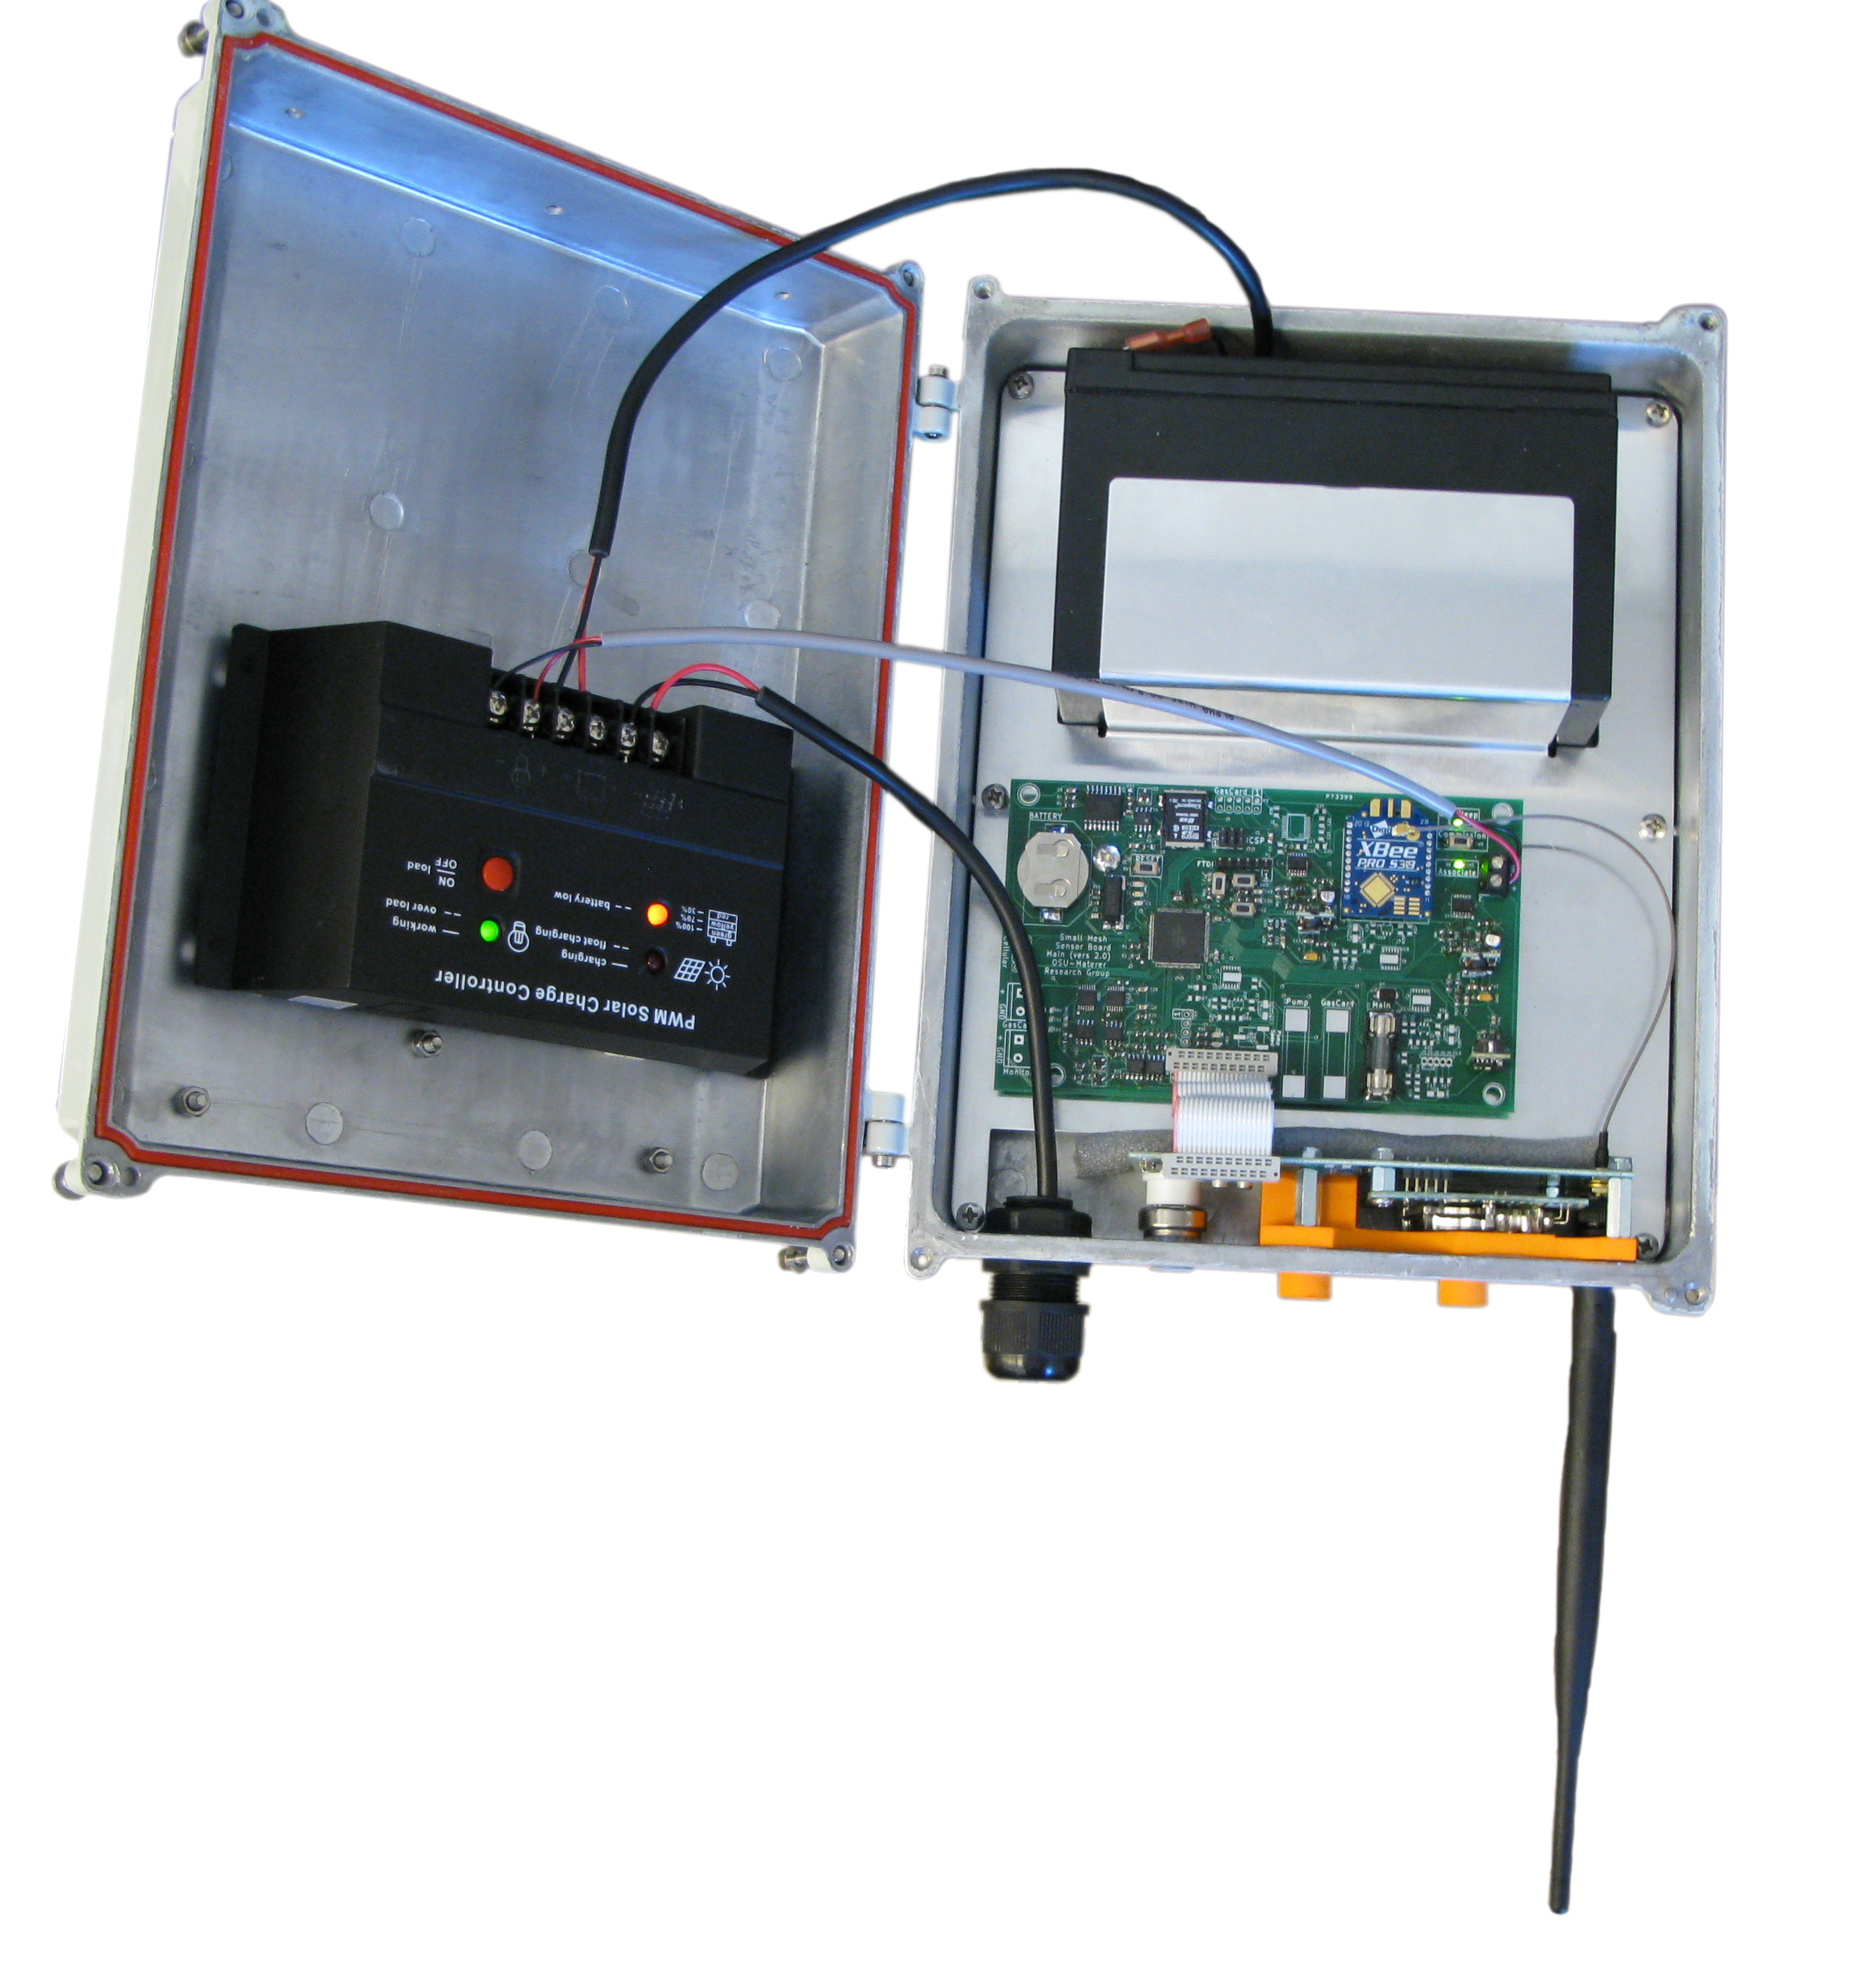
\includegraphics[width=.8\columnwidth,height=0.8\columnwidth,keepaspectratio]{testdeploy1.png}
			\caption[Completed Sensor Node]{A photo depicted the internal arrangement of boards and wiring within a completed sensor node.\label{fig:TLFig3_e}}
		\end{figure}
		
		A second generation prototype was developed replacing the Arduino and shield with a hand-soldered prototype of the final control board.  The updated internals of this board can be seen in Figure~\ref{fig:testdeploy2}.  This sensor unit was deployed in a residential section southwest of the Oklahoma State University main campus.  These tests showed that the printed circuit board functioned identically to the early Arduino prototype model.
		
		\begin{figure}[!t]
			\centering
			\includegraphics[width=.8\columnwidth,height=0.8\columnwidth,keepaspectratio]{testdeploy2.jpg}
			\caption[Internals of sensor node]{The completed sensor node was made by replacing the prototyping Arduino Mega with the custom circuit board designed for this project.  This shot of the internals shows the detail of the wiring between the components in the case.\label{fig:testdeploy2}}
		\end{figure}
		
	%\FloatBarrier
	\section{Mass Production}
	
		The circuitry for the individual units was produced in stages.  The sensor breakout board was printed and assembled early in the first quarter of 2015, the control board for both the communication and sensor nodes was printed and assembled in the \nth{3} quarter of 2015, and the cellular breakout board was printed early in the fourth quarter of 2015.  All printed circuit boards and pick-and-place assembly was contracted through Advanced Circuits in Aurora, Colorado.  The sensor boards, being designed first, were the first to be constructed.  These completed sensor boards were used during the Arduino prototyping phase so device design would employ the actual sensors.  This enabled development and honing of the serial communication with the sensors to and from the microcontroller.  The control boards were produced after several developing several prototypes and printed in a single batch.  Since the communication and sensor nodes utilize the same control board with different parts filled in, these boards were printed in a single batch.  The pick-and-place assembly of parts was done as two separate orders.  The cellular modem breakout board was only printed, due to the small number of parts required, and the simplicity of components.  These boards were hand-soldered.
		
		Construction of sensor nodes began in the beginning of the second quarter of 2015.   This final assembly phase was completed in waves of ten units at a time.  After the engineers assembled the nodes, the devices were given a quality control inspection and programmed.  The programmed sensor nodes were taken to the a proving ground north of campus and mounted on posts in sets of 10 sensor units.  Each of these sensor cohorts were networked with one of the prototype communication nodes and allowed to collect data for several weeks.  The data produced by the units were analyzed, and any device producing unsatisfactory results was taken for repair.  The final cohort was deemed satisfactory in the \nth{1} quarter of 2016.
		
		Construction of the communication nodes began near the end of the \nth{1} quarter in 2015.  Clear Lexan boxes were ordered to built by the OSU Civil Engineering mechanical shop to house the sensor breakout board for active sampling (see Section~\ref{sec:activesampling}).  Circuit boards were mounted to an orange back plate secured within the enclosure (Figure~\ref{fig:commbuild1}).  Only the top half of the plate was practical for mounting circuit boards, as the large batteries inside took up half of the volume of the enclosure.  Vinyl tubing was used to plumb the unit.  Input and output ports for gas were stuck through the bottom of the enclosure to pull gas from a location with a similar orientation to the passive interfaces on the sensor nodes.  The ports were placed on opposite ends of the bottom side of the enclosure to minimize recycling of gas which had already been analyzed.    Originally, the Lexan boxes were designed to easily disassemble in case modifications needed to be made on the sensor breakout board.  However, flow testing gas through the box showed that 36.2\% of the mass flow of gas through the entire system was being lost.  All of the joining edges of the clear plastic on the box, including the edge meant to be disassembled with screws, were sealed using dichloromethane in addition to silicone seals around the ribbon cable connection.  Each communication node was tested in the field, much like the sensor nodes, for quality assurance of the units.  
		
		\begin{figure}[!t]
			\centering
				\includegraphics[width=\columnwidth,keepaspectratio]{commbuild1.jpg}
				\caption[Components within the large communication nodes]{The layout of components within the large communication nodes.  The batteries take up most of the space inside the enclosure, so components were arranged to be bolted to the top of the back plate.\label{fig:commbuild1}}
		\end{figure}
		
		\begin{figure}
				\centering
				\includegraphics[width=\columnwidth,keepaspectratio]{commbuild2.jpg}
				\caption[Layout of board in communication nodes]{Behind the batteries, tubing to direct the air for the active sampling is laid.  Incoming air is passed through a filter and pumped through the clear box containing the sensor breakout board and the gas card sequentially before exiting the unit.\label{fig:commbuild2}}
		\end{figure}	
		
	%\FloatBarrier
	
	\section{Conclusions}
	
		The circuits described in this chapter come together to produce an effective set of sensing units.  The K-30 and MQ-4 gas sensors were applied to all units in the network.  For added accuracy for methane detection, a Gascard sensor has been added to the Tier 1 Communication Nodes.  This allows for the signals detected by the MQ-4 sensors on the network to be compared against a more reliable sensor to quantify potential concentration spikes.  The units are powered by switched 12V to 5V DC/DC converters which draw power from the enclosure's solar charged batteries.  The AVR processor issues commands to collect and store the data on the EEPROM memory and SD card backup.  The processor also handles power management by shutting down power intensive tasks such as the MQ-4's heater during periods of low battery voltage.  Communications between units are carried out by an XBee wireless radio with a limited range.  Communication nodes also incorporate a cellular modem breakout board which allows for communication of data across 3G cellular networks to a local server.  Individual sensors for gas concentration, pressure, temperature, and humidity measurements are incorporated onto a sensor breakout board which is mounted with access to the atmosphere.  The atmospheric interface is a passive sampling regime using a 3D printed part to protect delicate electronics for the low level sensor nodes.  The atmospheric sampling in communication nodes is an actively pumped regime to allow for the use of the 'flow-only' Gascard, and a special housing is used for the sensor breakout board to allow adaptation to this regime.  
		
		These individual parts working in concert allow for low-power operation, independent of human intervention for long periods of time.  The sensing devices are separated by sampling regime and location in the units, while wired to the storage architecture to collect the data.  The wireless networking capability of the units allows for the transfer and coordination of data.
		
		Devices have been produced in quantities of \textgreater100 units.  The increased production scale allows for these units to be produced cheaply.  The circuit boards and sensor infrastructure were assembled and programmed in batches during the \nth{1} quarter of 2016.  The testing of these units will be described in subsequent papers.  
	
	\bibliographystyle{unsrt}
	\bibliography{bib}

	\begin{appendices}
		\section{Fabrication Costs}
			\begin{table}[!t]
				\centering
				\caption{Fabrication Cost of Individual Units}
				\label{tab:onecosts}
				\begin{tabular}{cl|l|l}
					& Unit           & Sensor Node    & Comm. Node       \\ \hline 
					\multirow{3}{*}{Control Board} 
					& PCB            & \$\costonepcb  & \$\costonepcb    \\
					& Parts          & \$\costcparts  & \$\costcpartc    \\
					& Assembly       & \$\costcasyms  & \$\costcasymc    \\ \hline
					\multirow{3}{*}{Sensor Board}  
					& PCB            & \$\costonepcb  & \$\costonepcb    \\
					& Parts          & \$\costsparts  & \$\costsparts    \\ 
					& Assembly       & \$\costsasym   & \$\costsasym     \\ \hline
					\multirow{5}{*}{Sensors}       
					& MQ-4           & \$\costoneMQ   & \$\costoneMQ     \\
					& K-30           & \$\costoneK    & \$\costoneK      \\
					& Gascard        &                & \$\costoneGC     \\
					& Pumps          &                & \$\costonepump   \\
					& Lexan Box      &                & \$\costonelex    \\ \hline
					\multirow{2}{*}{Cell Board}    
					& PCB            &                & \$\costonepcb    \\
					& Parts          &                & \$\costcellpart  \\ \hline
					& Enclosure      & \$\costonetycsm& \$\costonetyclg  \\ \cline{2-4} 
					& \textbf{Total} & \$\costsumone  & \$\costsumtwo   
				\end{tabular}
			\end{table}
			
				\begin{table}[!t]
					\centering
					\caption{Fabrication Cost of Units Produced At Scale}
					\label{tab:sclcosts}
					\begin{tabular}{cl|l|l}
						& Unit           & Sensor Node    & Comm. Node       \\ \hline 
						\multirow{3}{*}{Control Board} 
						& PCB            & \$\costsclcpcb  & \$\costsclcpcb    \\
						& Parts          & \$\costsclcparts  & \$\costsclcpartc    \\
						& Assembly       & \$\costsclcasyms  & \$\costsclcasymc    \\ \hline
						\multirow{3}{*}{Sensor Board}  
						& PCB            & \$\costsclspcb  & \$\costsclspcb    \\
						& Parts          & \$\costsclsparts  & \$\costsclsparts    \\ 
						& Assembly       & \$\costsclsasym   & \$\costsclsasym     \\ \hline
						\multirow{5}{*}{Sensors}       
						& MQ-4           & \$\costsclMQ   & \$\costsclMQ     \\
						& K-30           & \$\costsclK    & \$\costsclK      \\
						& Gascard        &                & \$\costoneGC     \\
						& Pumps          &                & \$\costonepump   \\
						& Lexan Box      &                & \$\costonelex    \\ \hline
						\multirow{2}{*}{Cell Board}    
						& PCB            &                & \$\costsclcellpcb    \\
						& Parts          &                & \$\costsclcellpart  \\ \hline
						& Enclosure      & \$\costscltycsm& \$\costscltyclg  \\ \cline{2-4} 
						& \textbf{Total} & \$\costsumthr  & \$\costsumfou   
					\end{tabular}
				\end{table}
			
		\section{Y Events}
			\begin{table}[]
				\centering
				\caption{My caption}
				\label{tab:eventcount}
				\begin{tabular}{c|c|c|c|c|c|c}
					& \multicolumn{3}{l|}{Number of Carbon Dioxide Events} & \multicolumn{3}{l|}{Number of Methane Events} \\ \cline{2-7} 
					$x\left(\sigma\left(daily\right)\right)$ & y =1 hrs        & y =2 hrs        & y = 3 hrs        & y =1 hrs      & y =2 hrs      & y = 3 hrs     \\ \hline
					1           & 117             & 78              & 59               & 164           & 105           & 75            \\
					2           & 46              & {\color{red}33}              & 26               & 60            & {\color{red}35}            & 25           
				\end{tabular}
			\end{table}
	\end{appendices}
	
	%	% use section* for acknowledgment
	\section*{Acknowledgment}

	
\end{document}